\chapter{数据库设计}
\section{数据库环境说明}
{\color{red}
\subsection{检索速度v.s.稳定性}
本应用并不强调检索的速度,因为应用的数量并不会过多,所以更多地从稳定性考虑。

    从稳定性考虑,本系统的数据系统采用Oracle 12数据库系统;使用centOS作为
    操作系统。

\subsection{数据一致性考虑}
本系统同时也不强调一致性,应用的开发、应用的下载并不是冲突的操作。

用户下载的应用仅仅是系统中的最新版本即可。

}



\section{数据库的命名规则}
允许单词缩写,缩写的要求见表\ref{tab:abbr}

表名为单数,当前阶段设计的表有app,user,developer,people,dev\_app,user\_own\_app,comment.

字段无需加上前缀


\section{逻辑设计}
\begin{figure}[ht]
	\centering
	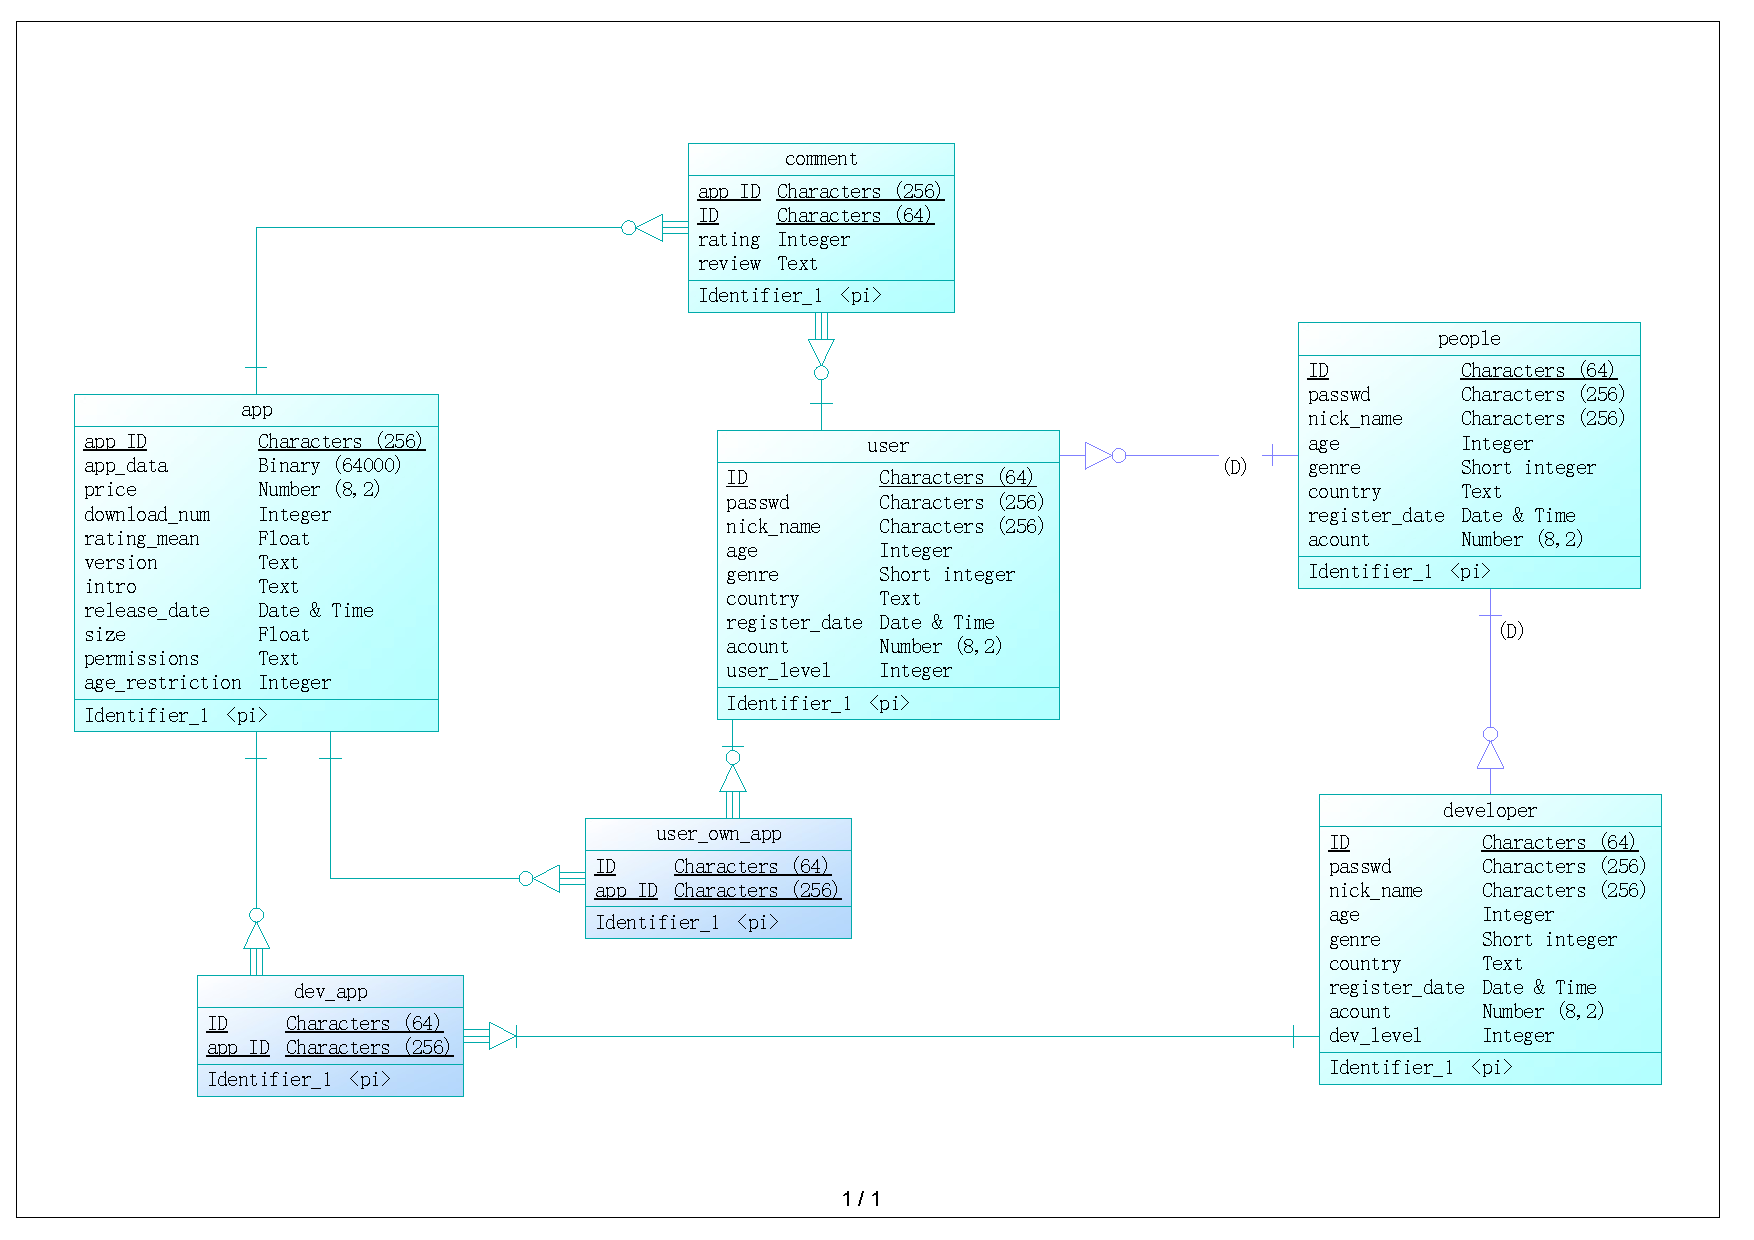
\includegraphics[width=16cm]{logical_data_model.pdf}
	\caption{逻辑模型图} \label{fig:logical_data_model.pdf}
\end{figure}
基本的实体关系逻辑模型见图\ref{fig:logical_data_model.pdf}



\section{物理设计}
\subsection{数据库产品}
使用oracle 12c数据库,要求是分布的且冗余。

\subsection{实体属性、类型、精度}
\subsubsection{app数据表设计}
\begin{table}[htbp]
\centering
\caption{app数据表Users设计} \label{tab:app_database}
\begin{tabular}{|c|c|c|c|c|}
    \hline
    字段名 & 类型 & 大小 & 说明 & 备注 \\
    \hline
    app\_ID & char & 256 & app的全局唯一标识符 & 主键 \\
    \hline
    app\_data & binary & $\cdot$ & app数据 & $\cdot$ \\
    \hline
    price & number & $\cdot$ & app的价格 & $\cdot$ \\
    \hline
    download\_num & int & $\cdot$ & 下载数量 & $\cdot$ \\
    \hline 
    rating\_mean & float & $\cdot$ & 平均评分 & $\cdot$ \\
    \hline
    version & text & $\cdot$ & 版本号 & $\cdot$ \\
    \hline
    intro & text & $\cdot$ & 简介 & $\cdot$ \\
    \hline
    release\_date & Date \& Time & $\cdot$ & 发行时间 & $\cdot$ \\
    \hline
    size & float & $\cdot$ & app数据大小 & $\cdot$ \\
    \hline 
    permissions & text & $\cdot$ & 权限要求 & $\cdot$ \\
    \hline
    age\_restriction & int & $\cdot$ & 用户年龄限制 & $\cdot$ \\
    \hline
\end{tabular}
%\note{用户数据表Users设计}
\end{table}

app表设计见图\ref{tab:app_database}

\subsubsection{user数据表设计}
\begin{table}[htbp]
\centering
\caption{user数据表设计} \label{tab:user_database}
\begin{tabular}{|c|c|c|c|c|}
    \hline
    字段名 & 类型 & 大小 & 说明 & 备注 \\
    \hline
    ID & char & 64 & 人员ID & 主键 \\
    \hline
    passwd & char & 256 & 加密后的密码 & $\cdot$ \\
    \hline
    nick\_name & char & 256 & 昵称 & $\cdot$ \\
    \hline 
    age & int & $\cdot$ & 年龄 & 考虑到年龄限制 \\
    \hline
    genre & char & 1 & 性别 & $\cdot$ \\
    \hline
    country & text & $\cdot$ & 国家 & 考虑到地域限制 \\
    \hline
    register\_date & Date\& Time & $\cdot$ & 注册时间 & $\cdot$ \\
    \hline
    acount & number & $\cdot$ & 账户金额 & $\cdot$ \\
    \hline
    user\_level & int & $\cdot$ & 用户的等级 & $\cdot$ \\
    \hline
\end{tabular}
%\note{订单数据表Orders设计}
\end{table}
user数据表设计见图\ref{tab:user_database}

\subsubsection{developer数据表设计}
\begin{table}[htbp]
\centering
\caption{developer数据表设计} \label{tab:developer_database}
\begin{tabular}{|c|c|c|c|c|}
    \hline
    字段名 & 类型 & 大小 & 说明 & 备注 \\
    \hline
    ID & char & 64 & 人员ID & 主键 \\
    \hline
    passwd & char & 256 & 加密后的密码 & $\cdot$ \\
    \hline
    nick\_name & char & 256 & 昵称 & $\cdot$ \\
    \hline 
    age & int & $\cdot$ & 年龄 & 考虑到年龄限制 \\
    \hline
    genre & char & 1 & 性别 & $\cdot$ \\
    \hline
    country & text & $\cdot$ & 国家 & 考虑到地域限制 \\
    \hline
    register\_date & Date\& Time & $\cdot$ & 注册时间 & $\cdot$ \\
    \hline
    acount & number & $\cdot$ & 账户金额 & $\cdot$ \\
    \hline
    dev\_level & int & $\cdot$ & 开发者的等级 & $\cdot$ \\
    \hline
\end{tabular}
%\note{订单数据表Orders设计}
\end{table}
developer数据表设计见表\ref{tab:developer_database}

\subsubsection{comment数据表设计}
\begin{table}[htbp]
\centering
\caption{comment数据表设计} \label{tab:comment_database}
\begin{tabular}{|c|c|c|c|c|}
    \hline
    字段名 & 类型 & 大小 & 说明 & 备注 \\
    \hline
    app\_ID & char & 256 & app的标识符 & 外键,来自app表\\
    \hline
    ID & char & 64 & 人员的ID & 外键,来自user表 \\
    \hline 
    rating & int & $\cdot$ & 评分& 0-5 \\
    \hline
    review & text & $\cdot$ & 评论 & $\cdot$ \\
    \hline
\end{tabular}
%\note{订单数据表Orders设计}
\end{table}
评论、评分数据表设计见表\ref{tab:comment_database}


\subsubsection{dev\_app数据表设计}
\begin{table}[htbp]
\centering
\caption{dev\_app数据表设计} \label{tab:dev_app_database}
\begin{tabular}{|c|c|c|c|c|}
    \hline
    字段名 & 类型 & 大小 & 说明 & 备注 \\
    \hline
    app\_ID & char & 256 & app的标识符 & 外键,来自app表\\
    \hline
    ID & char & 64 & 人员的ID & 外键,来自user表 \\
    \hline 
\end{tabular}
%\note{订单数据表Orders设计}
\end{table}
开发者开发的app表设计见表\ref{tab:dev_app_database}

\subsubsection{user\_own\_app数据表设计}
\begin{table}[htbp]
\centering
\caption{user\_own\_app数据表设计} \label{tab:user_own_app_database}
\begin{tabular}{|c|c|c|c|c|}
    \hline
    字段名 & 类型 & 大小 & 说明 & 备注 \\
    \hline
    app\_ID & char & 256 & app的标识符 & 外键,来自app表\\
    \hline
    ID & char & 64 & 人员的ID & 外键,来自user表 \\
    \hline 
\end{tabular}
%\note{订单数据表Orders设计}
\end{table}
用户拥有的(已购买或者已下载的)app表设计见表\ref{tab:user_own_app_database}

\section{安全性设计}
备份和容灾设计。

\section{数据库管理与维护说明}
对于数据库的维护,随时对数据库中的信息加以调试和保存备份。同样需要个工作人员进行系统的分析和用户的反馈,对系统进行升级以及功能的完善。同时保证系统安全有序的运行。